\makeatletter                                                   
\def\input@path{{../}}                                          
\makeatother                                                    
\documentclass[../main.tex]{subfiles}                           
\begin{document}                                                
\chapter{A 4th party logistics optimizer}
\label{ch:appr}
This chapter explains how we build our model, the fourth party logistics optimizer (4PLO).
The first section \cref{sec:alns}, desribes the meta heuristic approach 
The first \cref{sec:init} explain how we have chosen the initial solution.\par
Then \cref{sec:heur} present each of the heuristics included in the basic version of our model.
The next \cref{sec:choos}, explains how our model is choosing a heuristic in a given iteration. 
Then \cref{sec:weight} explain how our algorithm is using the performance history of heuristics to adapt the weights of the heuristics 

\Cref{sec:wild} present the wild escape algorithm used to prevent that our model gets stuck in a local optimum.

\section{ALNS for 4th party logistic problems}
\label{sec:alns}
Our metaheuristic is similar to the ALNS approach introduced by \cite{ropke06}, but we have adapted it to specifically solve our fourth party logistics problem. 
Our approach will be explained over the next few sections but the ALNS implementation differs mainly in the following way:
\begin{enumerate}
    \item Our heuristics each contain one removal and one insertion heuristic and are not chosen separately. 
    \item We integrate an escape algorithm to avoid that the algorithm gets stuck.
\end{enumerate}

A brief pseudocode of our implementation of ALNS for 4th party logistic problems is described in \cref{alg:alns}.  

\begin{algorithm}
    \label{alg:alns}
    \caption{ALNS for 4th party logistic problems}
    \begin{algorithmic}[1]
        \Function{alns}{}
        \State solution $s = generateInitialSolution()$
        \State solution $s_{best} = s$
        \State iterations since best solution found $i=0$
        \Repeat
            \If {$i>escape\ condition$}
                \State $s = wildEscape(s)$ 
            \EndIf
            \State $s' = s$
            \State select a heuristic, h, based on selection parameters
            \State $s' = applyHeuristic(h,s')$
            \If {$f(s') < f(s_{best})$}
                \State $s_{best}=s'$
            \EndIf
            \If {$accept(s', s)$}
                \State $s = s'$
            \EndIf
            \State update selection parameters and escape condition
        \Until {stop condition met}
        \State
        \Return $s_{best}$
        \EndFunction
    \end{algorithmic}
\end{algorithm}

The algorithm starts by picking an initial solution, and then moves into a loop where it picks a heuristic $h$, and an amount of orders $q$, before applying the heuristic to the current solution. 
It then updates the best solution and decides to accept the newly created solution or not until the stop condition is met.
At the start of the loop it checks if an escape condition is met where it will run \cref{alg:wild} on our current solution $s$. \par
We will now move on to explaining each step of the model more in detail.

\section{Initial Solution}
\label{sec:init}
Many different algorithms have been made for finding an initial solutions to a PDPTW. \cite{hosny12} found that the sequential construction sequence may be the most suitable construction algorithm for the MV-PDPTW. 
We have chosen to simply start with an initial solution where no orders are assigned to any vehicle, ie. all orders are assigned to the dummy vehicle in the solution permutation. 
We chose this because it is simple to implement, efficient in terms of running time and our model will be able to adapt to the problem on its own, regardless of the initial solution.

\section{Heuristics}
\label{sec:heur}
This section presents the heuristics used by our algorithm.
The first three heuristics7gc \ref{sec:swap}, \ref{sec:exch}, \ref{sec:2opt}, we call shuffeling heuristics. They try to quickly schuffle a given solution around to find new solutions in the same neighbourhood. \par

Removal and reinsertion heuristics are well reserached tools used in solving pickup and delivery problems. \cite{hemmati14} and \cite{hemmati16} use insertion and removal heuristics to solve benchmark tramp ship routing and scheduling problems and maritime shipping problems.
The last four heuristics, \ref{sec:rand}, \ref{sec:clust}, \ref{sec:greedy}, \ref{sec:shaw}, we refer to here as removal and reinsertion heuristics. Each of them contain one heuristic for removal and one heuristic for reinsertion.
These are used partly to move from one neighbourhood to another, and partly for local search depending on the amount of solution elements, $q$, being reinserted.  

\subsection{Swap}
\label{sec:swap}
This heuristic simply tries to swap the pickup and delivery of two different orders until the first time it finds a fit. 
\cref{fig:swap} illustrates a successful swap between two orders in a simple solution permutation. 

\begin{figure}                                                                                     
 \centering                                                                                     
 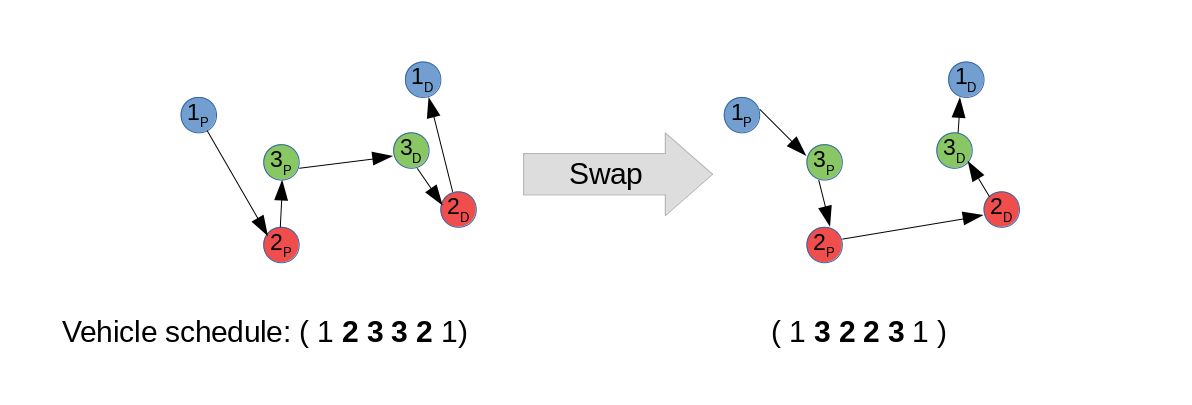
\includegraphics[width=\textwidth]{swap_ill.png}                                     
 \label{fig:swap}                                                                            
 \caption{A swap heuristic performed on a simple solution with two orders. The numbers indicate an order and the letters P and D indicate pickup and delivery respectively.}
\end{figure}

This heuristic is very efficient and jumps randomly around a neighbourhoods solution space.

\subsection{3-exchange}
\label{sec:exch}
The 3-exchange heuristic selects a random vehicle with at least two assigned orders, and performs an exchange of 3 assigned positions until a feasible new combination is found. A 3-exchange of position 2, 4 and 6 in a simple permutation is illustrated by \cref{fig:exch}. \newline

\begin{figure}                                                                                     
 \centering                                                                                     
 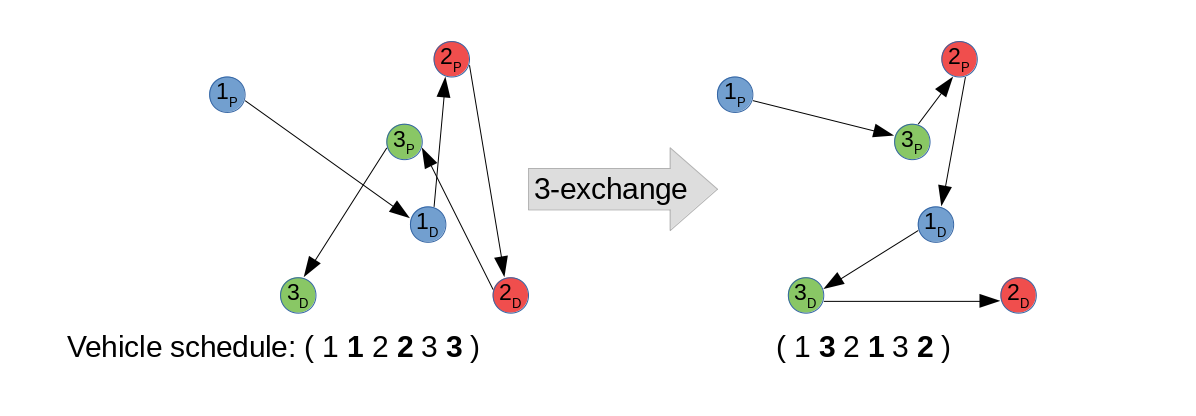
\includegraphics[width=\textwidth]{3-exchange_ill.png}                                     
 \label{fig:exch}                                                                            
 \caption{A 3-exchange heuristic performed on a simple solution with three orders. The numbers indicate an order and the letters P and D indicate pickup and delivery respectively.}
\end{figure}

This heuristic is very fast, as the exchanges are fast operations and checking if a vehicles schedule is feasible is also a very effective operation. Like the swap heuristic from the previous section this heuristic jumps randomly around a neighbourhoods solution space.

\subsection{2-opt}
\label{sec:2opt}
2-opt is a common heuristic used in travelling salesman problems aswell as with metaheuristics to solve VRP. \cite{lin65} implemented the 2-opt heuristic for travelling salesmen problem and \cite{bullnheimer99} combined 2-opt with the ant system metaheuristic.
The 2-opt heuristic used in this paper is similar to the heuristic from \cite{carrabs07}.
\Cref{fig:2opt} illustrates one iteration of our 2-opt heuristic on a simple permutation.

\begin{figure}                                                                                     
 \centering                                                                                     
 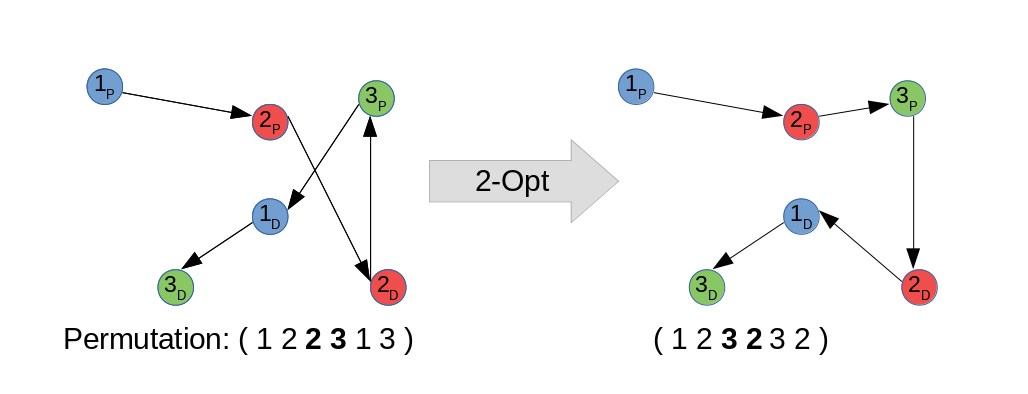
\includegraphics[width=\textwidth]{2-opt_ill.png}                                     
 \label{fig:2opt}                                                                            
    \caption{One 2-opt heuristic operation performed on a simple solution with three orders. In this example $i=2$ and $j=4$ so the schedule $S_{ij}$ is reversed. The numbers indicate an order and the letters P and D indicate pickup and delivery respectively.}
\end{figure}

\begin{algorithm}
    \label{alg:2opt}
    \caption{2-opt heuristic}
    \begin{algorithmic}[1]
        \Function{twoOpt}{$S\in \{ solution \ schedules \}$}
        \Repeat
        \State $S_{best} = S$
        \For{$i<S.length$}
            \State $j=i+1$
            \For{$j<S.length$}
                \State schedule $ S' = S_{0i} + reverse(S_{(i+1)j}) + S_{(j+1)n}$ 
                \If {$f(S')<f(S_{best})$} 
                \State $S = S'$
                \EndIf
            \EndFor
        \EndFor
        \Until {no further improvement found}
        \State 
        \Return $S$
        \EndFunction
    \end{algorithmic}
\end{algorithm}


The heuristic selects a random vehicle with more than 2 orders.
For the selected vehicle it divides up the route of the vehicle in 3 parts. 
All orders up until the index $i$ of the vehicle route are inserted normally. 
Orders from the index $j+1$ until the end of the route are also inserted normally. 
Then finally orders from the index i+1 until index j are inserted in reverse order.
If the new schedule has a smaller cost than the original schedule, the schedule is remembered as the new best route. 
When all reverses have been performed on the current route, the best route is selected as the new route.
This operation is continued until no improvement can be made ie. the best possible schedule for the selected vehicle has been found.


\subsection{Remove random and insert first fit}
\label{sec:rand}
Removes randomly between 2 orders and 10 percent of the amount of orders and reinserts them randomly in their first possible position. 
This heuristic is used to jump from one neighbourhood to another and is trying to search for possible solutions regardless of the cost they produce.

\subsection{Remove non-clustered and insert clustered}
\label{sec:clust}
This heuristic tries to remove orders that are bundled together but belong to different clusters. It then tries to bundle orders together in the best possible way.
The orders pickup and delivery locations are all assorted into clusters based on the distance between them. 
We use a hirarchial single linkage clustering algorithm to cluster locations together into $k$ clusters. (TODO: make algorithm table for herarchial single linkage algorithm) 
Then we compare each set of $k$ cluster to eachother using the siluette coefficient, and keep the best one. (TODO: make algorithm table for siluette coefficient) \newlinw \par
To choose which order to remove we have ranked the orders based on how many clusters are shared within a vehicles schedule.
If an orders pickup and delivery shares no cluster with any other pickup or delivery nodes the rank is 0. 
If the order shares the same cluster with both pickup and delivery node as all other pickup and delivery nodes within a vehicle it is given a rank 1.  
This leads us to quite easily differenciate between a well clustered order and a not well clustered one.
The orders are sorted based on their rank and we choose the order to pickup that has the lowest rank, using some randomization, based on the value $p$. 
We choose the order on the position $k^p$ in the rank where k is a random number. 
We have chosen $p=4$ in this paper.  \newline \par
To reinsert the orders we have chosen to try and maximize the cluster rank we introduced above. This means we find the vehicle where the rank is the highest and insert the order in the best possible position in the chosen vehicle. 

\subsection{Remove Worst and Insert Greedy}
\label{sec:greedy}
Removing orders in the most costful positions and reinserting it in its cheapest (greedy) position seems to be a reasonable way of moving towards a better solution.
We therefore propose a heuristic that removes the orders with the highest cost $C_{i}$.
The $C_i$ is calclated as the increase in a vehicles schedule cost with the chosen order.
We remove orders again based on the same randomness factor explained above. We do this by first ranking the orders based on cost and choose the order in the $k^p$ position. \newline \par
The reinsertion is using a greedy algorithm where it simply checks to find the best possible possition for the order and inserts it there. 
\newline 
\subsection{Remove Similar and Regret Insert}
\label{sec:shaw}
The removal heuristic used in this heuristic is based on \citet{shaw97} with slight modifications based on our problem. 
It removes orders that share specific similar qualities, as the basic idea is that by replacing these orders by eachother we find new, hopefully better, solutions. 
Another good reason to remove similar orders is that it could be advantagous to reinsert these orders togther on the same vehicle since they share alot of the same properties in regards to distance, time etc.
We define a relatedness factor $r_{ij}$ which represents how much the order $i$ is related to the order $j$. 
The lower the value of $r_{ij}$ the more the two orders $i$ and $j$ are related.
The relatedness of two orders we base here on the following properties: 
a distance property, a weight property, an overlapping timewindow property, a property indicating if the same vehicles can be used to serve each request, and finally if the orders belong to the same factory.

The relatedness factor is given by the following equation:

\begin{equation}
\label{relatedness}
    r_{ij} = \psi ( D_{i j} + D_{(i+n)(j+n)}) + \omega|Q_i - Q_j|
    + \phi (1-\dfrac{|V_i\cap V_j|}{max(|V_i|, |V_j|)} ) + \tau G_{ij} + \chi (U_{ij} + U_{(i+n)(j+n)})
\end{equation}

$D_{ij}$, $Q_i$, are defined in the problem formulation section and these values have been normalised to result in a value between $[0..1]$. 
$V_i$ is the set of vehicles that can serve order $i$. 
The parameter $G_{ij}$ is 1 if $i$ belong to another factory than $j$ and 0 if they belong to the same factory. 
$U_{ij}$ is the timewindows at the pickup and delivery location, equal to 0 if the two orders have identical time windows and 1 if not. It corresponds to the sum of overlapping time windows divided by the overlapping span of the two time window sets.
It can be formulated as follows
\begin{equation}
    \label{overlaptime}
    U_{ij} = 1 - 
\dfrac{ 
    \sum\limits_{\substack{p\in \pi_i\\ o\in \pi_j\\ \underline{T_{ip}}\leq \overline{T_{jo}}\\ \underline{T_{jo}}\leq\overline{T_{ip}}}} 
    (\min(\overline{T_{ip}}, \overline{T_{jo}}) - \max(\underline{T_{ip}},\underline{T_{jo}}) )
    }
    {\max{(\max\limits_{p\in \pi_i} \overline{T_{ip}}, \max\limits_{o\in \pi_j} \overline{T_{jo}})} - 
    \min{(\min\limits_{p\in \pi_i} \underline{T_{ip}}, \min\limits_{o\in \pi_j} \underline{T_{jo}}}) -     
    \sum\limits_{\substack{p\in \pi_i\\ o\in \pi:q_j\\ \underline{T_{ip}}\geq \overline{T_{j(o-1)}}\\ \underline{T_{jo}}\geq\overline{T_{i(p-1)}}}} 
    (\min(\underline{T_{ip}}, \underline{T_{jo}}) - \max(\overline{T_{i(p-1)}},\overline{T_{j(o-1)}}) ) 
    }
\end{equation}

Here $\overline{T_{ip}}$ and $\underline{T_{ip}}$ are the upper and lower time windows defined in the problem formulation.
Thus the relatedness measure is given a value $0\leq r_{ij} \leq 2\psi + \omega + \phi + \tau  + \chi$. 
We have chosen the following values in this paper $\psi=0.7$, $\omega=1.0$, $\phi=0.8$, $\tau=0.3$, $\chi = 0.3$. \newline\par
The insertion part of this heuristic tries to improve on the insert greedy by calculating a regret value, $c^*_i$, which represents how much is lost by inserting this order in its second best position.

\section{Choosing a heuristic}
\label{sec:choos}

\section{Adaptive weight adjustment}
\label{sec:weight}

\section{Acceptance criteria}
\label{sec:accept}

\section{Wild escape algorithm}
\label{sec:wild}
Algorithms containing large neighbourhood heuristics, such as our model, are known to be good at searching locally aswell as globally. 
However they do sometimes get stuck in one neighbourhood, and it is important that our algorithm is able to react automatically in these situations.
If we for 500 iterations find no improvement in the solution we are assuming that we are stuck. In this case we need to do something to get unstuck. 
We have designed our algorithm so that in the case when no improvement in found for 500 iteration, we run \cref{alg:wild} with the stopping criteria of 10 iterations. iterations apart from the normal iterations, where we accept any new solution found regardless of the objective value. 
In these iterations we use what we call a wild escape algorithm.
The algorithm is described in \cref{alg:wild}.
We use the heuristics7gc from \cref{sec:rand}, \cref{sec:exch} and \cref{sec:swap} as these heuristics are not trying to improve and select targeted solutions but rather returns the first feasible solution they find. 
We also increase the amount of elements the heuristics7gc are working on to effectively move further then the normal search iterations. 

\algsetup{
    linenodelimiter=\ 
}
\begin{algorithm}
    \label{alg:wild}
    \caption{Wild escape}
    \begin{algorithmic}[1]
        \Function{wildEscape}{s}
        \Repeat
        \State $s=applyRandomWildHeuristic(s)$;
        \Until stop condition met
        \EndFunction
    \end{algorithmic}
\end{algorithm}

\biblio                                                         
\end{document}
